\documentclass{article}
\usepackage{graphicx}

\title{A Game of Pinching Pennies}
\author{Edward Yu}

\begin{document}

\maketitle
\epigraph{Life is like a puzzle. The more you try to resolve it, the more you will get trapped in the mystery.\dots}{Rahul Singh}

That is exactly how I felt after seeing the “weekend puzzle” sent to my school’s math team one Friday afternoon in January. Our longtime math coach, Mr. Dean Ballard, had introduced the puzzle a few weeks ago not only to us math team members, but also to the whole world via the Riddler, a column of the prestigious news analysis website FiveThirtyEight. First published in ``ye olden days'' back in 1907, it is a simple game with rules that anyone can understand:

Alex has some number of pennies, which Bill divides into two piles. They take turns, with Alex going first. Each turn, a player either removes any number of pennies from one pile, or an equal number of pennies from both piles. Taking nothing is not allowed.

\begin{center}
     
\includegraphics[scale=0.8]{images/play_game.png}
\end{center}

The winner will be the one who takes the last penny. Since, of course, Alex and Bill are both geniuses, they will play perfectly to optimize their chances of winning. What numbers of pennies can Alex choose at the beginning to guarantee a win?


In fact, Mr. Ballard says this game was once a bonus problem for his sixth-grade math class. I (and some friends), veteran high-school math enthusiasts, will certainly have no problem solving this… right? As it turns out, I was stumped by this problem for several days, and almost anyone would be challenged to solve it. One student who struggled with the game described: “There must be a pattern – I know it. I just can’t see it.” This sums up the agony of working on such a seemingly easy problem.


Mr. Ballard was not trying to train the Math Team to become future gamblers, nor was he trying to make con artists out of us. Instead, as a passionate puzzle-lover, he is bringing us to see the connections between an obscure game and a well-known pattern.
As for the real answer to the puzzle, it is surprisingly related to the famous Fibonacci numbers: 1, 1, 2, 3, 5, 8, 13…, where each number is the sum of the previous two—and has a much deeper relation to the golden ratio, $\phi = \frac{1+\sqrt{5}}2$.
\begin{center}
    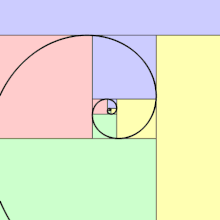
\includegraphics[scale=0.45]{images/fibonacci_seq.png}
\end{center}

Mr. Ballard himself also had some comments on the puzzle. He finds it interesting “because there are surprises in it; you start with the simple rules of a game, and you realize that you’ve discovered another way of generating the Fibonacci numbers”—which turn out to be hidden in the set of winning stone-piles for Bill (the second player). In addition, Mr. Ballard notes that, “just from looking at the puzzle, you would never see the Fibonacci numbers or the golden ratio.”

\epigraph{The connections between things…these connections are delightful discoveries in math.}{Mr. Dean Ballard}

Many math puzzles are like this – countless trials of seemingly random games, endless rows of numbers marching down the page. From the fractal symmetry of snowflakes to the golden-ratio spirals of mollusks to the geometric structure of the buckminsterfullerene molecule, nature hints us with simple yet intricate patterns, guiding us towards elegant perfection. After a long period of head-scratching, wall-punching, or muttered obscenities, you might at last find the answer.


So, go play the game with friends or family. You might get to solve one of the mysteries in your life, and who knows: you might even get to (re)visit sixth-grade math again.

\begin{center}
    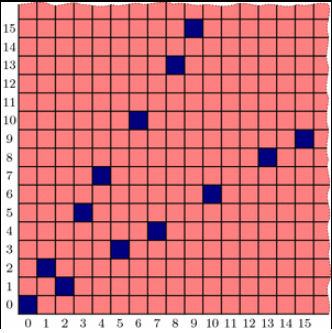
\includegraphics[scale=0.8]{images/wythoff_game.png}
\end{center}

Comment: if you’re curious to learn more about the game, it’s called Wythoff’s Game of Nim. First studied by W. A. Wythoff in 1907, it gained popularity after being featured in Martin Gardner’s famous Scientific American column, “Mathematical Games.”
\end{document}